\chapter{Evaluation}
\label{evaluation-chapter}

In this chapter, we evaluate our model and compilation strategy, using
several approaches.
First, we consider what assurances can be gained from mechanisation of
the model and proofs of the compilation rules.
In addition, we compare code produced by our strategy to that produced by
icecap, using some examples to evaluate the strategy.
% TODO: more that we can add here?
We note, finally, that the process of constructing the model already
embeds important validation effort, via numerous reviews of the
standard, and close interaction with the standardisation committee,
which led to some changes to the standard.

Next, in Section~\ref{mechanisation-of-models-section}, we consider
the assurances gained from mechanisation of the models that form the
starting point of the strategy.
In Section~\ref{proofs-of-laws-section}, we discuss the proofs of the
compilation rules used in the strategy and how they provide assurances
of the correctness of the strategy.
Afterwards, in Section~\ref{tool-support-section}, we consider
mechanisation of the strategy and then, in
Section~\ref{examples-section}, we evaluate the strategy with some
examples.
Finally, we conclude in
Section~\ref{evaluation-final-considerations-section}.


\section{Mechanisation of Models}
\label{mechanisation-of-models-section}

% TODO: rephrase this
The correctness of our compilation strategy relies on the correctness
of the models used as input to the compilation strategy.
Their correctness relies on the inputs to the models meeting the
assumptions made in Section~\ref{compilation-assumptions-section}.
If these assumptions are not met, then the behaviour of model is not
correct and the compilation strategy cannot be applied.
For example, if the sequence of instructions in the program causes the
operand stack to overflow the maximum stack size, the invariant of
$StackFrame$ is violated and program's behaviour is chaotic.
Our compilation strategy cannot be applied to such a program, since no
stack slots are created beyond the maximum stack size to handle such a
situation in the strategy, and it is not clear what the expected C
code would be.

As discussed in Section~\ref{cee-validation-section}, the fact that
the models are written in CZT ensures they have correct syntax and
types.
CZT performs this checking continuously and flags up errors as they
occur, so they can be quickly corrected during the writing of the
models.

We have also performed some proofs on the Z schemas defining the
semantics of the bytecode instructions, using Z/EVES 2.4.1 with CZT as
its user interface.
There are two main groups of results.
The first is domain check proofs, ensuring partial functions are
not applied outside their domain.
These are proof obligations generated by Z/EVES, and so do not have
corresponding theorems stated.
These proofs are not required for schemas that do not directly
reference partial functions.

The second group of results is precondition proofs.
These require that a final state exists for the schema, which ensures
that the requirements of the schema are not contradictory.
Stating and proving these theorems also extracts the preconditions of
the operations, since those must be stated as assumptions of the
theorems.

The preconditions we have found include those required to avoid
operand stack overflows and underflows, that local variable indices
are within the range of the local variable array, and that
program-address updates do not go outside of the current method's
bytecode array.
These conditions are ensured by standard JVM bytecode verification,
which we assume inputs to the strategy pass.
The existence of at least one stack frame is also required for
bytecode instructions to execute, and this property is ensured by the
condition on the loop in the $Running$ action.

A further precondition required by the interpreter operations is that
the value $cs$ is such that the class and method in which a program
address occurs is unique.
This condition is required to ensure that the current class and method
can be uniquely determined from the value of $pc$.
This is required by the invariant of $InterpreterState$, but need only
be fulfilled as a precondition when a new stack frame is created,
since it can be ensured from the invariant on the initial state for
the other operations.
This condition on $cs$ is reasonable since the bytecode instructions
for each method should be at separate addresses in $bc$.

% TODO: these proofs will be removed in the main thesis
The statements of the theorems proved can be found in
Appendix~\ref{stack-frames-theorems-appendix} and
Appendix~\ref{interpreter-theorems-appendix}, with their corresponding
proofs in Appendix~\ref{stack-frames-proofs-appendix} and
Appendix~\ref{interpreter-proofs-appendix}.
We have also proved various additional lemmas in the course of
constructing these proofs.
Those which are specific to the model are listed along with the
precondition theorems in Appendix~\ref{stack-frames-theorems-appendix}
and Appendix~\ref{interpreter-theorems-appendix}.
Some of them are general facts that could be of use in other theorems,
which are listed in Appendix~\ref{additional-lemmas}.

\section{Proofs of Laws}
\label{proofs-of-laws-section}

The correctness of our compilation strategy is ensured by the
correctness of the individual compilation rules.
We prove these rules in terms of algebraic laws, whose correctness is
known.
This gives assurance that no step of the compilation strategy involves
applying a transformation that changes the semantics of the input
program.

We adopt an algebraic style of proof, in which the algebraic laws are
applied one-by-one to transform the left-hand-side of a rule into its
right-hand-side.
This ensures that the term obtained in each step of the proof is shown
to be a refinement of, or equal to, that of the previous step, by
application of a known law.
The overall proof then follows from the transitivity of refinement.
Thus, every step of the proof is justified formally and this can be
easily seen from the layout of the proof.

The laws used in the proofs come from various sources.
Some are existing laws taken from~\cite{oliveira2006}
and~\cite{miyazawa2012}, which have already been proved as part of
those works, and so can be safely reused.
We have also used a few ZRC laws from~\cite{cavalcanti1998}, which can
be applied to \Circus{} since the semantics of ZRC are compatible with
those of \Circus{}, by Theorem 4.3 from~\cite{oliveira2006}.
Standard least-fixed-point laws, stated in~\cite{hoare1998} are also
applied to \Circus{} recursion, since it defined using
least-fixed-points.
Some laws follow as a trivial consequence of the definitions given in
these sources, such as Law~[\nameref{action-intro-law}], which follows
from the definition of process refinement, which does not reference
actions not used in the main action of a process.

We have proved other laws using the proof assistant
Isabelle~\cite{nipkow2002} with its implementation of
UTP~\cite{foster2015}.
The constructs supported by that implementation limit the types of
laws that may be proved, but we have proved several laws relating to
conditionals, assumptions, and assignment.
In the case of conditionals, we contributed an implementation of
\Circus{} conditionals to Isabelle/UTP.
This has allowed us to prove laws more general than those that have
been proved previously, since previous laws have used the fact that
conditionals can be converted to external choice, which requires that
the guards be disjoint and provide complete coverage.
We require these more general laws to perform transformation of the
$Running$ action during the elimination of program counter, since not
all program counter values have a corresponding bytecode instruction,
so we cannot ensure coverage.
Our work on this has now been integrated into Isabelle/UTP itself.

Some of the algebraic laws are applied directly in our strategy, and
may be found in
Appendix~\ref{compilation-strategy-algebraic-laws-section} after the
compilation rules specific to each stage of the strategy.
A full list of the algebraic laws used in this thesis, including both
those used in our compilation strategy and those used in the proofs of
the compilation rules, can be found in
Appendix~\ref{algebraic-laws-appendix}.

% discuss compilation rules and their proofs
% explain the importance of the algebraic proof style
% explain source of laws used for proofs

\section{Tool Support}
\label{tool-support-section}

In addition to proving the individual compilation rules, it also is
useful to be able to automatically generate the code resulting from
the strategy in order to validate it.
This allows for consideration of the issues involved in handling
actual SCJ programs and shows how the strategy as a whole fits
together to produce the final code.
It also facilitates the consideration of examples, which provide
additional validation of the strategy.

We have thus created a simple prototype to transform SCJ class files
to corresponding \Circus{} models generated by the strategy.
This prototype is written in Java, using the Apache bytecode emulation
library for reading class files so that real output from the standard
Java compiler can be used directly.
It outputs the \Circus{} code for the $CThr$ process that results from
applying the compilation strategy to the input files.
We focus on this part of the C code model, and the first two stages of
the strategy that generate it, as it is quite complex and so most
benefits from review of the code produced.

The data refinement of memory is comparatively simple, since it just
involves collecting the fields for each class and producing the
corresponding \Circus{} code from the strategy.
Its correctness is sufficiently ensured by the correctness of the
compilation rules, so we do not handle it in our prototype.

\begin{figure}[p]
  \begin{center}
    \begin{tikzpicture}
      % \begin{class}{ClassFileModelConverter}{0,0}
      %   \operation{+ \uline{main(args : String[])}}
      % \end{class}

      \umlclass{Model}{
        $\cdots$
      }{
        + toModelString() : String \\
        + doEliminationOfProgramCounter() : ThrCFModel \\
        - methods() : HashSet\textless{}FullMethodID\textgreater{} \\
        - allMethodsSeparated(newModel : ThrCFModel) : boolean \\
        $\cdots$
      }

      \umlclass[x=-3.5cm,y=-3.2cm]{ClassModel}{$\cdots$}{$\cdots$}

      \umlclass[x=3.5cm,y=-3.2cm,type=abstract]{BytecodeModel}{}{}

      \umlclass[alias=aconstnull,x=8cm,y=-2cm]{ACONST\_NULL}{$\cdots$}{$\cdots$}
      \node at (8cm,-3.8cm) {\Huge  $\vdots$};
      \umlclass[x=8cm,y=-6cm]{RETURN}{$\cdots$}{$\cdots$}

      \umlinherit[geometry=-|-]{aconstnull}{BytecodeModel}
      
      \umlinherit[geometry=-|-]{RETURN}{BytecodeModel}

      \umluniaggreg[geometry=|-,anchor1=-110,arg2=classes,mult2=0..*,pos2=1.4,arm2=-0.1cm]{Model}{ClassModel}
      \umluniaggreg[geometry=|-,anchor1=-90,arg2=bytecodes,mult2=0..*,pos2=1.6,arm2=-0.1cm]{Model}{BytecodeModel}

      \umlclass[x=0cm,y=-7.8cm]{ThrCFModel}{
        $\cdots$
      }{
        + addMethod(name : FullMethodID, actions : CircusAction[]) \\
        + toModelString() : String \\
        + doEliminationOfFrameStack() : CThrModel \\
        - getReturnAction(CircusAction[] actions) : CircusAction \\
        - introduceReturnAction(actions : CircusAction[], \\
        $\t1$ returnAction : CircusAction) : CircusAction[] \\
        - returnActionDist(actions : CircusAction[]) : CircusAction[] \\
        %- eliminateNewStackFrame(actions : CircusAction[], \\
        %$\t1$ methodReturnsValue : HashMap\textless{}FullMethodID, Boolean\textgreater{}) : CircusAction[] \\
        %- eliminateVarBlocks(actions : CircusAction[]) : CircusAction[] \\
        $\cdots$
      }

      \umluniaggreg[geometry=|-|,anchor1=130,arg2=classes,mult2=0..*,pos2=2.8,arm1=0.4cm]{ThrCFModel}{ClassModel}

      \umlclass[x=0cm,y=-13cm,type=abstract]{CircusAction}{}{
        \umlvirt{+ expandWithClassInfo(classInfo : ClassModel) : CircusAction} \\
        \umlvirt{+ doEFSDataRefinement(stackDepth : int) : CircusAction[]} \\
        $\cdots$
      }

      \umlclass[alias=handleaconstnullepc,x=7cm,y=-15.5cm]{HandleAconst\_nullEPC}{
        $\cdots$
      }{
        $\cdots$
      }
      \node at (7cm,-17.3cm) {\Huge  $\vdots$};
      \umlclass[x=7cm,y=-19.5cm]{Assignment}{
        $\cdots$
      }{
        % + getVar() : String \\
        % + getExpr() : String() \\
        $\cdots$
      }

      \umlinherit[geometry=-|,anchor2=-20]{handleaconstnullepc}{CircusAction}
      
      \umlinherit[geometry=-|,anchor2=-20]{Assignment}{CircusAction}

      \umluniaggreg[geometry=|-|,anchor1=-90,arg2=methodActions,mult2=0..*,pos2=2.8]{ThrCFModel}{CircusAction}

      \umlclass[x=0cm,y=-17cm]{CThrModel}{
        $\cdots$
      }{
        + toModelString() : String \\
        $\cdots$
      }

      \umluniaggreg[geometry=|-|,anchor1=90,arg2=methodActions,mult2=0..*,pos2=2.8]{CThrModel}{CircusAction}
      
      % \aggregation{Model}{classes}{0..*}{ClassModel}
      % \aggregation{Model}{bytecodes}{0..*}{BytecodeModel}
    \end{tikzpicture}
  \end{center}
  \caption{Class diagram for our implementation of the compilation
    strategy}
  \label{implementation-class-diagram-figure}
\end{figure}

To ensure we get the most benefit from our prototype, we follow the
strategy and the form of the compilation rules as closely as possible
in its design, shown in
Figure~\ref{implementation-class-diagram-figure}.
Our implementation of the compilation strategy validates our reasoning
in designing it, since the code generated for the examples has the
expected form matching that of the icecap compiler.

Some of the classes used in our implementation and the relationships
between them are shown in
Figure~\ref{implementation-class-diagram-figure}. 
Our prototype begins by reading each input class file and extracting
the information into \texttt{ClassModel} and
\texttt{BytecodeModel} classes.
\texttt{ClassModel} represents the $Class$ type from our model and
makes available all the information represented in that type.
\texttt{BytecodeModel} is an abstract class whose subclasses represent
individual bytecode instructions; it represents the $Bytecode$ type
from our model.
The set of \texttt{ClassModel} structures and array of
\texttt{BytecodeModel}s are collected together into a \texttt{Model},
representing the inputs to the compilation strategy.

The application of the first stage of the compilation strategy to a
\texttt{Model} is initiated by invocation of its
\texttt{doEiminationOfProgramCounter()} method.
This returns a \texttt{ThrCFModel} object, which represents the
$ThrCF$ process generated from the inputs represented by the
\texttt{Model}.
The \texttt{doEiminationOfProgramCounter()} method applies each step
of Algorithm~\ref{epc-algorithm}.
It begins by replacing each bytecode instruction with the \Circus{}
actions that result from applying bytecode expansion to it, as
described in Algorithm~\ref{expand-bytecode-algorithm}.
We represent \Circus{} actions by subtypes of an abstract class
\texttt{CircusAction}.
These subtypes represent both general \Circus{} constructs such as
variable blocks, conditionals and assignment, and references to
specific actions in our model, such as the $Handle{*}EPC$ actions.

The sequences of actions produced by bytecode expansion are placed
into an array of arrays of \texttt{CircusAction}s, representing the
branches of the choice over $pc$ in $Running$.
We test the types of the actions in these sequences to check if they
match the compilation rules of the strategy, and update the sequence
of actions in a branch accordingly, in order to perform the
introduction of sequential composition
(Algorithm~\ref{introduce-forward-sequence-algorithm}), introduction
of loops and conditionals
(Algorithm~\ref{introduce-loops-and-conditionals-algorithm}), and
method resolution (Algorithm~\ref{resolve-method-calls-algorithm}).

We also construct a control-flow graph, which we use to guard the
application of some rules as indicated in the strategy, and which is
reconstructed after the application of a compilation rule.
The sequence of actions corresponding to entry point of a method whose
control-flow graph consists of a single node are added to the
\texttt{EPCModel} during method separation
(Algorithm~\ref{separate-complete-methods-algorithm}), with their $pc$
assignments removed when they are added, to produce the result of
Algorithm~\ref{pc-elimination-algorithm}.
The refine main actions step
(Algorithm~\ref{refine-main-actions-algorithm}) operates on the
$Started$ and $MainThread$ actions, which have a known form, so we
simply output the form resulting from this step, instantiated with the
method names collected in the strategy.

The application of the elimination of frame stack stage to the
\texttt{ThrCFModel} is performed by its
\texttt{doEliminationOfFrameStack()} method, which returns a
\texttt{CThrModel} representing the $CThr$ process generated after
this stage.
In our implementation we apply the rules of this stage by traversing
the actions of each method, checking for actions that match the form
of the rules.
Rules that operate on sequences of more than one rule are applied by
private methods of \texttt{ThrCFModel}, whereas those that affect only
a single action are applied by methods of the \texttt{CircusAction}
classes.
We group together the application of similar rules in some of these
methods.

The removal of launcher returns
(Algorithm~\ref{remove-launcher-returns-algorithm}) is performed by
first obtaining the return action with a \texttt{getReturnAction()}
method, which corresponds to the \Call{ReturnAction}{} function
referenced on line~\ref{algorithm-determine-return-action} of
Algorithm~\ref{remove-launcher-returns-algorithm}.
The return action is then introduced after infinite loops in the by a
method \texttt{introduceReturnActions()}, which performs the
exhaustive application of Law~[\nameref{rec-action-intro-law}] on
line~\ref{algorithm-introduce-infinite-loop-returns}, and distributed
using a method \texttt{returnActionDist()}, which performs the
exhaustive application of Rule~[\nameref{conditional-dist-rule}] on
line~\ref{algorithm-distribute-return}.
The remainder of this stage is upon the $ExecuteMethod$, $Started$ and
$MainThread$ actions, whose forms are known, so we simply output the
resultant forms for them at the end of the application of the
strategy.
The return actions within the body of a method are refined to the
corresponding data operations by this step so we take them to refer to
those data operations in subsequent steps.
Although the return actions are distributed outside the method actions
in this step, they are moved back inside the method actions in the
next step, so we do not perform this moving in the implementation.

During the localise stack frames step
(Algorithm~\ref{localise-stack-frames-algorithm}), the data refinement
on line~\ref{algorithm-remove-currentClass-data-refinement} of
Algorithm~\ref{localise-stack-frames-algorithm} only affects the
definition of the process' data operations, not the \Circus{} code for
the methods of our program, so it does not need to be explicitly
performed in our implementation.
We instead begin localising the stack frames by calculating the number
of arguments for each method as specified on
lines~\ref{algorithm-numArgs-declaration}
to~\ref{algorithm-static-args-check-end} of
Algorithm~\ref{localise-stack-frames-algorithm}, and then refining
each method by adding parameters as specified by
Rule~[\nameref{arguments-introduction-rule}] and a $stackFrame$
variable block as specified by
Rule~[\nameref{HandleReturnEPC-stackFrame-introduction-rule}].
These are added directly to each method's actions, since the
parametrised block is moved inside the method by the procedure called
on line~\ref{algorithm-redefine-method-action-to-include-parameters}.
After this, the $InterpreterNewStackFrame$ operations are eliminated
from the body of each method by a method
\texttt{eliminateNewStackFrame()}, because they are moved into inside
the methods whose references follow them and refined to stack frame
initialisation operations.

In the introduce variables step, the \texttt{expandWithClassInfo()}
method of \texttt{CircusAction} applies the rules on
lines~\ref{algorithm-apply-refine-PutfieldSF}
to~\ref{algorithm-apply-refine-NewSF} of
Algorithm~\ref{introduce-variables-algorithm}, which make use of
information on the value of $frameClass$.
The data refinement on line~\ref{algorithm-local-data-refinement} is
performed by \texttt{doEFSDataRefinement()}, passing the depth of the
operand stack at each point in the method based on the rules in
Algorithm~\ref{introduce-operandStack-assumptions-algorithm}.
Finally, \texttt{eliminateVarBlocks()} applies the rules on
lines~\ref{algorithm-apply-eliminate-value1-value2-conditional-rule}
to~\ref{algorithm-argument-variable-elimination} of
Algorithm~\ref{introduce-variables-algorithm}, which eliminate extra
variable blocks around various constructs.
The removal of the $frameStack$ from the state
(Algorithm~\ref{remove-frameStack-from-state-algorithm}) is trivial
and has no effect on the method actions so there is nothing to be done
for it in our implementation.
The \Circus{} model resulting from this stage is extracted as a
\texttt{String} from the \texttt{CThrModel} and written to an output
file.

As our prototype is just for the purposes of validating the strategy,
we have not performed a direct formal verification of its
implementation.
However, since we have applied the compilation rules in the
implementation in a way that matches the form of the rules in the
strategy, which are proved, we are confident of its correctness.
The correctness of the implementation is further validated by loading
the output of the prototype into CZT to ensure that it is well-formed,
and checking the output to ensure it has the expected form.
% since the loop and conditional
% introduction rules operate on assignments of the form
% $pc := \IF b \THEN x \ELSE y$, and so are agnostic to the condition
% checked.

% TODO: rephrase to account for stuff moved to next section
There have been various considerations raised in producing this
prototype. 
One consideration is that of how to represent the class, field,
and method identifiers used in the bytecode.
In the model these are represented by given sets, since their
representations do not matter provided they can be distinguished from
one another and information necessary to the operation of the strategy
(specifically, the number of arguments to a method identifier and
whether it denotes an instance initialisation method) can be gleaned
from them.
For simplicity, we just use the identifier strings supplied in the
input Java class files, concatenating method and field names with
their type signatures, and removing or replacing characters that are
not valid in \Circus{} identifiers.
% However, many of these identifiers are quite long, since they use
% fully qualified class names, so we generally shorten them when
% presenting examples, provided the identifiers are still unique.
% The shortenings performed are generally elimination of packages names
% from class names, and removal of type signatures from method
% identifiers when two methods do not have the same name (initialisation
% method identifiers have a shortened version of their class name
% prepended to distinguish them).

Since we apply the compilation rules in our implementation as
prescribed in our strategy, we can observe how the individually
correct compilation rules fit together.
It has highlighted the need to consider the extent of
variable blocks.
In particular, the loop and conditional introduction rules must match
the variable block introduced by the expansion of the
\texttt{if\_icmple} bytecode instruction. 

We also found that Rule~[\nameref{resolve-normal-method-rule}] must
extend the $poppedArgs$ variable block to cover the reference to the
method action it introduces, in order to match the combination of
$IntepreterNewStackFrame$ operation and method action reference in
Rule~[\nameref{arguments-introduction-rule}].
In addition, it revealed that the return action must be distributed
outside of the variable blocks surrounding conditionals in
Rule~[\nameref{conditional-dist-rule}].
The form of the methods resulting from the elimination of program
counter also made clear the need for $Poll$ actions before $Running$
in $Started$ and $MainThread$, in order to match method calls
introduced in the body of methods.

All these considerations have been taken into account in the strategy
presented in the previous chapter.
In the next section, we discuss some examples whose compilation we
have automated using our prototype. 
We focus on the generated code, and its relation to icecap results.

% discuss mechanisation of strategy
% explain considerations surrounding bytecode subset
% explain what confidence this brings

\section{Examples}
\label{examples-section}

In this section, we evaluate the strategy by considering some examples
of SCJ programs.
We compare the code generated from the prototype implementation of the
compilation strategy to that resulting from the icecap HVM for each of
the examples.
The examples we choose are taken from those developed during the
high-integrity Java applications using \Circus{}
project~(which may be found at~\url{www.cs.york.ac.uk/circus/hijac/case.html}).
We particularly focus on some SCJ Level 1 examples that illustrate
some main features of SCJ.

We have run the examples through both our prototype and the icecap
compiler.
Our main focus here is validating the compilation of the SCJ programs
themselves, which is separate from the SCJ infrastructure it depends
on.
However, the SCJ infrastructure includes the SCJ API, which is written
in Java.
Since icecap and our strategy both operate on complete SCJ programs,
including the Java code called by the program, the SCJ API must be
included in the code compiled.
This is shown in
Figure~\ref{program-infrastructure-compilation-figure}, which shows
the structure of an SCJ program in relation to the infrastructure and
compilation.

How much of the SCJ API implementation is written in Java, and hence
included in the code that undergoes compilation, depends upon the
services provided by the operating system and virtual machine.
These are generally accessed through native method calls in Java code,
but are usually implementation-defined and not visible to end-users,
indicated by the dashed line in
Figure~\ref{program-infrastructure-compilation-figure}.
The infrastructure in our model is accessed via special methods
representing these native methods, but our model of the SCJ
infrastructure is intended to model a wider part of the SCJ
infrastructure than that which icecap implements in C.
In order to account for these differences when passing the examples
through the compilation strategy, we provide a small implementation of
part of the SCJ API, linking the SCJ code of the examples to the SCJVM
via the special methods in our model.
This does not affect the correctness of the examples or the validity
of comparing them, since the SCJ API is the same for both icecap and
our implementation; it is only the implementation of the API that
differs.
Ensuring the correctness of the API implementation is a separate
issue, work on which has begun in~\cite{freitas2016}, so we do not
consider it here.
In the compiled code, the code corresponding to the methods of the SCJ
API is separate to the code corresponding to the methods of the SCJ
program, as indicated in
Figure~\ref{program-infrastructure-compilation-figure}, so they can be
easily distinguished.

% In order to best compare the code generated from the examples, we have
% tried to keep the code passed to icecap and our strategy as similar as
% possible but, since much of the SCJ infrastructure relies on direct
% interaction with the SCJVM to provide features such as scheduling and
% memory management, we have provided our own library covering part of
% the SCJ API.
% Our implementation of the SCJ API is generally a quite thin layer,
% providing the required classes of SCJ and linking the SCJ code to the
% SCJVM via the special methods in our model, which represent native
% methods in the Java code.
% Much of the SCJ infrastructure is already represented in our model by
% the $Launcher$ and SCJVM services, so it is not necessary to provide
% code for it in our SCJ API implementation.
% The API we provide is the same as that for icecap, so the compilation
% results for the code of the examples themselves are similar.

\begin{figure}[t]
  \centering
  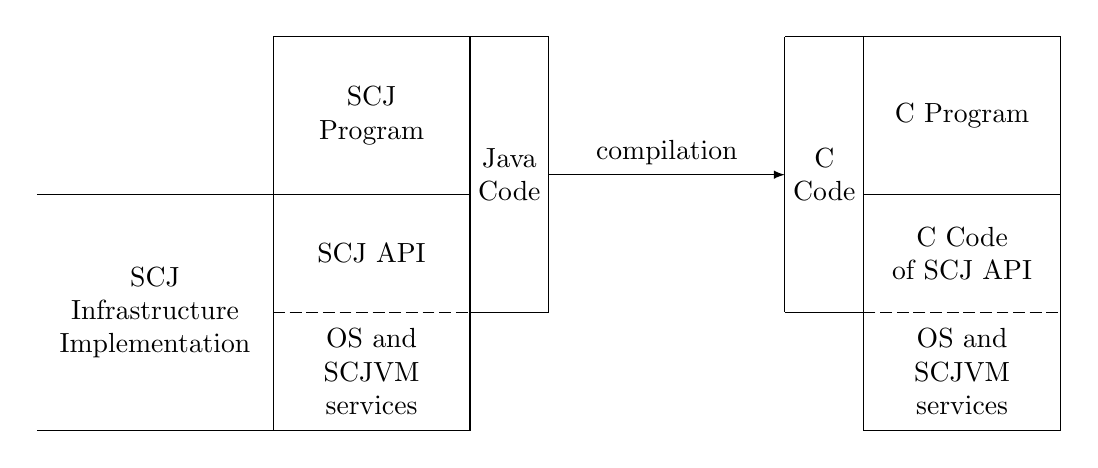
\begin{tikzpicture}
    \path (0,0) -- (0,5)
    node[pos=0.0] (bottom) {}
    node[pos=0.3] (machineBoundary) {}
    node[pos=0.6] (codeBoundary) {}
    node[pos=1.0] (top) {};

    \path (0,0) -- (10,0)
    node[pos=-0.3] (left) {}
    node[pos=0.00] (preCompilationLeft) {}
    node[pos=0.25] (preCompilationRight) {}
    node[pos=0.35] (JavaRight) {}
    node[pos=0.65] (CLeft) {}
    node[pos=0.75] (postCompilationLeft) {}
    node[pos=1.00] (postCompilationRight) {}
    node[pos=1.00] (right) {};

    \draw (bottom -| preCompilationLeft) rectangle (top -| preCompilationRight);
    \path (bottom -| preCompilationLeft) rectangle (machineBoundary -| preCompilationRight) coordinate[pos=0.5] (PreVM);
    \draw[dashed] (machineBoundary -| preCompilationLeft) rectangle (machineBoundary -| preCompilationRight);
    \path (machineBoundary -| preCompilationLeft) rectangle (codeBoundary -| preCompilationRight) coordinate[pos=0.5] (PreAPI);
    \draw (codeBoundary -| preCompilationLeft) rectangle (codeBoundary -| preCompilationRight);
    \path (codeBoundary -| preCompilationLeft) rectangle (top -| preCompilationRight) coordinate[pos=0.5] (PreCode);

    \node[align=center] at (PreVM) {OS and\\SCJVM\\services};
    \node[align=center] at (PreAPI) {SCJ API};
    \node[align=center] at (PreCode) {SCJ\\Program};

    \draw (bottom -| left) -- (bottom -| preCompilationLeft);
    \draw (codeBoundary -| left) -- (codeBoundary -| preCompilationLeft);
    \path (bottom -| left) -- (codeBoundary -| preCompilationLeft) coordinate[pos=0.5] (SCJVM);
    \node[align=center] at (SCJVM) {SCJ\\Infrastructure\\Implementation};

    \draw (top -| preCompilationRight) -- (top -| JavaRight);
    \draw (machineBoundary -| preCompilationRight) -- (machineBoundary -| JavaRight);
    \path (machineBoundary -| preCompilationRight) -- (top -| JavaRight) coordinate[pos=0.5] (JavaCode);
    \draw (machineBoundary -| JavaRight) -- (top -| JavaRight) coordinate[pos=0.5] (JavaCodeMid);
    \node[align=center] at (JavaCode) {Java\\Code};
    
    \draw (bottom -| postCompilationLeft) rectangle (top -| postCompilationRight);
    \path (bottom -| postCompilationLeft) rectangle (machineBoundary -| postCompilationRight) coordinate[pos=0.5] (PostVM);
    \draw[dashed] (machineBoundary -| postCompilationLeft) rectangle (machineBoundary -| postCompilationRight);
    \path (machineBoundary -| postCompilationLeft) rectangle (codeBoundary -| postCompilationRight) coordinate[pos=0.5] (PostAPI);
    \draw (codeBoundary -| postCompilationLeft) rectangle (codeBoundary -| postCompilationRight);
    \path (codeBoundary -| postCompilationLeft) rectangle (top -| postCompilationRight) coordinate[pos=0.5] (PostCode);

    \node[align=center] at (PostVM) {OS and\\SCJVM\\services};
    \node[align=center] at (PostAPI) {C Code\\of SCJ API};
    \node[align=center] at (PostCode) {C Program};

    \draw (top -| CLeft) -- (top -| postCompilationLeft);
    \draw (machineBoundary -| postCompilationLeft) -- (machineBoundary -| CLeft);
    \path (machineBoundary -| postCompilationLeft) -- (top -| CLeft) coordinate[pos=0.5] (CCode);
    \draw (machineBoundary -| CLeft) -- (top -| CLeft) coordinate[pos=0.5] (CCodeMid);
    \node[align=center] at (CCode) {C\\Code};
    
    \draw[-latex] (JavaCodeMid) -- node[above] {compilation} (CCodeMid);
    
  \end{tikzpicture}
  \caption{The relation of an SCJ program to the SCJ infrastructure
    in compilation}
  \label{program-infrastructure-compilation-figure}
\end{figure}

There are various issues with the compilation strategy and our
prototype that we identified and fixed while considering these
examples.
The first is that the examples make use of bytecode instructions that
are not in the representative subset of instructions described in
Section~\ref{cee-bytecode-subset-subsection}.
However, since this is a representative subset, the strategy can be
easily expanded to handle the missing instructions by analogy to the
instructions in the subset.
For example binary operation bytecodes can have their semantics
defined in a similar way to \texttt{iadd}, with compilation rules to
handle them similar to those for \texttt{iadd} (and their
corresponding proofs similar).
Conditional instructions can be handled in a similar way to
\texttt{if\_icmple} during bytecode expansion, and subsequently
handled by existing compilation rules.

Array instructions are slightly more challenging to replicate in the
strategy, but can be represented in programs using classes that
contain the individual slots of the array as fields. 
These fields can then be accessed using methods that select the
appropriate field with conditionals over an array index.
A full implementation would replace these method calls with
specialised communications with the struct manager, which would handle
them using C arrays.
Although this would require changes to the object/struct manager, it
would be relatively simple in terms of the strategy as the structure
of the arrays would not change during compilation and very little
would need to be performed on the instructions in the interpreter.

We also found that $poppedArgs$ variable block around special method
calls is not eliminated in
Algorithm~\ref{introduce-variables-algorithm}, although normal methods
are handled by Rule~[\nameref{method-parameter-introduction-rule}] and
Rule~[\nameref{poppedArgs-sync-elim-rule}].
Eliminating $poppedArgs$ around special methods requires rules similar
to these rules for to handle each individual special method.
We have not added these to the compilation strategy itself due to
space constraints, but the rules required are simple rules to
substitute the value of $poppedArgs$ into the body of the action and
then eliminate the variable block with the initialisation of
$poppedArgs$.

% illustrate with some examples
% compare to icecap

%TODO: finish general explanation about examples

\subsection{\texorpdfstring{\texttt{PersistentSignal}}{PersistentSignal}}

Our first example is \texttt{PersistentSignal}. 
It consists of a single mission with two event handlers:~a periodic
handler, \texttt{Producer}, and an aperiodic handler, \texttt{Worker}.
These communicate through an instance of a third class,
\texttt{PersisentSignal}, after which the example is named.
The \texttt{PersisentSignal} class contains a boolean flag, with
\texttt{synchronized} methods to read, set and clear it.
\texttt{Producer} releases clear the \texttt{PersistentSignal} flag, and then signals
for the \texttt{Worker} to release.
The \texttt{Worker} sets the \texttt{PersistentSignal} flag during its
release and the \texttt{Producer} checks the flag to see if the
\texttt{Worker} has finished its release.
Both the \texttt{Producer} and \texttt{Worker} produce output to
indicate when they are released.

The main purpose of this example is to demonstrate SCJ's scheduling
behaviour.
The priority of the \texttt{Worker} is set higher than the priority of
the \texttt{Producer}, so the \texttt{Worker} always preempts the
\texttt{Producer}, leaving the flag set at the end of its release
before allowing the \texttt{Producer} to finish its release.
This means that the synchronisation applied to the methods of
\texttt{PersistentSignal} may not be necessary, but it is good
practice due to the possibility of release jitter whereby the
scheduler may switch to a thread after a small delay if, for example,
the scheduler is running on its own thread or in response to clock
interrupts.

The code generated by our prototype for this example is similar to
that generated for it by icecap.
The operations on local variables and the operand stack are
represented by operations on C variables in both the code icecap
generates and the code resulting from our strategy. 
The names of the variables differ between icecap and our
implementation, since icecap uses the local variable names from the
original SCJ code, which are included in class files for debug
purposes, but different names can be used without affecting the
correctness of the code.

The synchronisation behaviour is particularly evident in this example,
and is handled the same in both the code from icecap and the code from
our prototype.
The lock is taken just before a call to a synchronized method, and
released at the end of the synchronized method.
In our model this is represented by the $takeLock$ and $releaseLock$
channels; icecap uses a \texttt{handleMonitorEnterExit()} function to
handle both, passing a boolean flag to it to distinguish between taking
the lock and releasing the lock.
The objects locked on are the same in our code as for icecap:~the
first argument on the stack when calling the method, and the first
local variable when returning from the method.

There are some differences, most of which apply to all the examples
discussed in this section.
The code from icecap has extra code to throw and handle exceptions,
which we do not consider in our model since SCJ code can be checked to
ensure exceptions will not be thrown.
Handling of exceptions in our strategy is a possibility for future
work, although it is not necessary for any of our examples.

Jumps in the bytecode are translated by icecap using \texttt{goto}
statements in C.
This allows bytecode instructions to be translated more directly, but
it means the resulting code is not fully MISRA-C compliant.
In our compilation strategy, we avoid the use of \texttt{goto} by
considering the control-flow graph of each method and introducing
structures such as loops and conditionals.
This has the added advantage of making the resulting code more
readable and, since we have have certainty that this transformation
does not change the semantics of the code, it is not necessary to use
the most direct translation as icecap does.

The icecap code uses many additional variables, most of which are used
to temporarily hold values indicating whether an exception has been
thrown.
It also has a stack pointer variable, which is passed to each method
(in addition to the method's arguments) and used, in addition to the
other variables, to hold some values so that the compiled code can be
mixed with interpreted code.
As this feature is not required in our work, we do not include a stack
pointer in the code generated by our compilation strategy.
The cases where extra variables are eliminated in our strategy are
matched by icecap, such as comparing variables representing stack
slots directly in conditionals, rather than copying them into
intermediate variables, which are removed by
Rule~[\nameref{eliminate-value1-value2-conditional-rule}] in our
strategy.

\subsection{\texorpdfstring{\texttt{Buffer}}{Buffer}}

Our second example is \texttt{Buffer}, which, like the previous
example, consists of two event handlers:~a periodic handler,
\texttt{Producer}, and an aperiodic handler, \texttt{Consumer}.
During a release of \texttt{Producer}, it calls the
\texttt{executeInOuterArea()} method of \texttt{ManagedMemory},
passing in an anonymous \texttt{Runnable} object stored in a field
\texttt{\_switch} of \texttt{Producer}.
The \texttt{run()} method of the object in \texttt{\_switch} allocates
an instance of \texttt{Object} and stores it in a field \texttt{data}
of \texttt{Producer}.
Since it is executed via \texttt{executeInOuterArea()}, this instance
of object is allocated in the memory area outside the per-release
memory for \texttt{Producer}, which is the mission memory.
The object in \texttt{data} is then stored in a buffer and the
\texttt{Consumer} is released, which pops the object from the buffer.

The purpose of this example is to demonstrate the memory behaviour of
SCJ.
Since the object passed via the buffer is used by both event handlers,
it must be allocated in mission memory to ensure that it is available
to both event handlers.
Since objects are, by default, allocated in an event handler's
per-release memory area during its release, this allocation must be
performed via \texttt{executeInOuterArea()}.
The buffer itself must also be allocated in mission memory, but it
does not require use of \texttt{executeInOuterArea()}, since it is
allocated during mission initialisation.
Since the mission memory is not cleared during the mission, it would
eventually run out of space to allocate the objects with repeated
releases of \texttt{Producer}.
To prevent this, the \texttt{Producer} maintains a count of how many
times it has been released and does not allocate the object or store
it in the buffer if it has been released more than a set number of
times.

The code generated from this example has many of the same
characteristics we have already described for the
\texttt{PersistentSignal} example.
In particular, the methods of the buffer are synchronized, so
synchronisations are produced in the code around calls to such
methods.
In addition, we make some further considerations related to the how
the use of the \texttt{executeInOuterArea()} method is represented in
the code.
The call to \texttt{executeInOuterArea()} itself is a simple static
method call in both the code generated by icecap and the code
generated by our strategy, since the SCJ API does not differ between
them.
Although the implementation of the method differs between the icecap
code and the code from our strategy, due to the differing SCJ
libraries used, they both contain code to change the memory area, a
call to the \texttt{run()} method of the \texttt{Runnable} object
passed into the method, and code to change the memory area back to its
previous value.

The call to the \texttt{run()} method of the \texttt{Runnable} object
is interesting as many classes in the SCJ infrastructure implement
\texttt{Runnable}, providing a large set of possible targets for the
call.
There is a large difference in the set of targets chosen for the
method call by icecap and our prototype --- the icecap code lists 10
targets, whereas our code lists 4.
The only target that appears on both lists is \texttt{Producer\$1},
the anonymous class in \texttt{Producer} that is the actual target of
the \texttt{executeInOuterArea()} call we are considering.
The other three targets in our code are all subclasses of
\texttt{AsyncEventHandler}, which is part of the superclass hierarchy
for event handlers. 

\texttt{AsyncEventHandler} is included in the list of choices for
icecap and is selected there by searching the superclasses of the
object the method is called on until one of the listed targets is
found.
In our code, we adopt a different approach, selecting using the
object's actual type but directing the call to the class in which the
method is defined.
This means that while there are three branches of the choice
corresponding to subclasses of \texttt{AsyncEventHandler}, the
contents of those branches are the same call to
\texttt{AsyncEventHandler}'s \texttt{run()} method.
This is simply a static resolution of the superclass search that
icecap conducts, for each of the possible subclasses of
\texttt{AsyncEventHandler} in the example program, so it may be
regarded as equivalent.
The other targets listed in the icecap code are parts of the SCJ
infrastructure that are handled in our model by the $Launcher$ and
SCJVM services.

%TODO: say something about how targets are chosen here?

\subsection{\texorpdfstring{\texttt{Barrier}}{Barrier}}

Our third example is \texttt{Barrier}, which demonstrates a common
pattern in real-time systems, where an event only happens when
multiple event handlers have signalled their readiness.
It is based around a class named \texttt{Barrier}, which implements
this pattern.
There are three types of event handlers in this
example:~\texttt{FireHandler}, which is the type of aperiodic event
handlers that must signal their their readiness to the
\texttt{Barrier}, \texttt{LaunchHandler}, the aperiodic handler that
releases when all the \texttt{FireHandler}s have signalled their
readiness, and \texttt{Button}, a periodic handler that simulates
events releasing the \texttt{FireHandler}s.
In the example, two instances of \texttt{FireHandler} are created,
with corresponding \texttt{Button} event handlers:~one that releases
every 2 seconds, and one that releases every 9 seconds.

When a \texttt{FireHandler} releases, it checks if it has already
triggered the \texttt{Barrier}, and calls a method of the
\texttt{Barrier} to trigger it if it has not already been triggered,
passing a numerical identifier.
When the \texttt{Barrier} is triggered, it sets a boolean flag
corresponding to the passed numerical identifier, then checks if all
the boolean flags are set.
When all the boolean flags are set, the \texttt{Barrier} releases its
associated \texttt{LaunchHandler} object and resets all the boolean
flags.
The \texttt{LaunchHandler} gives output to indicate when it is
released.

This example shows a more complex scheduling behaviour than that of
the previous examples.
The \texttt{FireHandler} and \texttt{LaunchHandler} event handlers
have higher priority than the \texttt{Button} event handlers, so they
cannot be interrupted by the periodic events firing.
However, the \texttt{FireHandler} and \texttt{LaunchHandler} handlers
have the same priority, and the methods of \texttt{Barrier} are
synchronized, so the boolean flags in \texttt{Barrier} are completely
reset before the \texttt{LaunchHandler} executes.
Due to the differing periods for the \texttt{Button} handlers, the
first \texttt{FireHandler} releases four or five times before the second
\texttt{FireHandler} releases and \texttt{LaunchHandler} executes.

A particular feature of interest in the code generated for this
example stems from the fact that it has multiple aperiodic event
handler types.
This means that a release of an aperiodic handler in our code (as may
occur when the \texttt{Barrier} is triggered) is represented by a
choice between them, although both branches of the choice contain a
call to the \texttt{release()} method of
\texttt{AperiodicEventHandler}.
The corresponding icecap code simplifies this to a direct call to the
\texttt{release()} method of \texttt{AperiodicEventHandler}, omitting
the unnecessary choice.
Such a transformation could be made in our strategy, although fully
applying it involves eliminating the $getClassIDOf$ communication used
to get the class identifier used in the choice.
As explained in
Section~\ref{compilation-final-considerations-section}, this requires
operating on multiple processes and so we leave it to future work.
Note that the fact that there are multiple instances of
\texttt{Button} and \texttt{FireHandler} makes no difference to either
the code from icecap or the code from our strategy.

\section{Final Considerations}
\label{evaluation-final-considerations-section}